%!TEX root = ../thesis-guntur.tex
%************************************************
\chapter{Experimental Setup}
\label{ch:experimental-setup} % $\mathbb{ZNR}$
%************************************************

TODO:
- separate context, setup
- add metrics explicitly:
	- correlation (rho) and p value, explain what it is and what it does
	- how to validate the model: RMSE, residual error, percentage of total population


% The previous chapters present the bla bla.
% \marginpar{Use this to write down some comments.}
In this chapter we present the method of the experiments to collect the data. We first start with the investigation of \ac{MAC} address randomization behavior. Then we discuss the main experiment, which is about examining the correlation between the level of social density and smartphone sensor readings. Lastly, we present the method of data extraction from collection of raw log files.

\section{MAC Address Randomization} % (fold)
\label{sec:mac_address_randomization}
In this first setup we are interested in seeing the behavior of \ac{MAC} address randomization. This phenomenon is observed in both Android and iOS devices~\cite{thesis061}. By using this randomization technique, the devices will randomize its \ac{MAC} address in each particular circumstances to increase the privacy of the user and thus making the current people tracking technology no longer works~\cite{thesis079}. We need to investigate \ac{MAC} address randomization behavior because we will use the \ac{MAC} address counting as a proxy to estimate the level of social density. \ac{MAC} address randomization is a potential threat to this approach. 

In this experiment, we exploit the active scanning mechanism of WiFi, in which each WiFi-enabled device is required to broadcast probe request packets to scan for available WiFi \ac{AP}~\cite{thesis082}. In the probe request, a piece of unique information exists, e.g., the device's \ac{MAC} address and supported WiFi modes, which indicates where the probe request packet comes from. We capture the probe request packets from nearby WiFi-enabled devices and store the captured information to a log file.

The randomized \ac{MAC} address uses locally administered address, which is indicated by the second-least-significant bit of the first octet of the address~\cite{thesis082}. The original \ac{MAC} address uses universally administered address, which is uniquely assigned by its manufacturer.

In this experiment we take note on 
\begin{enumerate*}[label={\alph*)},font={\color{red!50!black}\bfseries}]
  \item the timing when the randomized MAC address appears,
  \item the \ac{SN} field\footnote{The \ac{SN} field is a 12-bit field indicating the sequence number of a probe request packet. This marks the order of how the packets are broadcasted.} of the packet,
  \item and the variation of the \ac{MAC} address.
\end{enumerate*}

We investigate the randomization behavior in both iOS, using iPad mini with iOS 10.0, and Android, with LG Nexus 5X with Android 6.0 (Marshmallow). When experimenting on iPad mini, we turn the LG Nexus 5X off, and vice versa, to make sure that each device is not disturbing each other. We do this experiment within 30 minutes for each device.

We choose a remote area where we cannot detect any other probe request except from our device to perform the experiment. We use Wireshark\footnote{\url{https://www.wireshark.org}}, a popular network protocol analyzer software, to capture and store the captured probe request packets to a \verb|pcap| file. We run this experiment on Apple's MacBook Air with built-in WiFi card that supports monitor mode.

% residual information
% http://repo.thehackademy.net/depot_madchat/racine/reseau/wireless/IDS/wlan-mac-spoof.pdf
% http://blogs.cisco.com/wireless/apple-ios-8-and-mac-randomization-what-it-means-for-ciscos-connected-mobile-experiences-cmx-solution
% http://community.arubanetworks.com/t5/AAA-NAC-Guest-Access-BYOD/iOS-8-amp-MAC-Address-Randomization/td-p/169900
% http://www.cso.com.au/article/547177/apple_randomises_mac_addresses_ios_8_killing_off_key_ad-tracking_tool/
% http://www.imore.com/closer-look-ios-8s-mac-randomization
% https://en.wikipedia.org/wiki/MAC_address










\section{Correlation between Crowd Count and Sensor Readings} % (fold)
\label{sec:crowd_count_correlation}
% intro, aim, and how we achieve the aim
In this experiment we are interested to see the correlation between the number of people in the surroundings and the sensor readings. We collect the data in different conditions to see the trend of the correlation. Correlation between smartphone sensor readings and people count indicates that smartphone sensor readings are possible means to estimate the level of social density in the surroundings. However, we have to be aware of the strength of the correlation. We are also interested to see the trend of the variables, i.e., is it negative or positive correlation.

In this section we start with the method we use to count or estimate the crowd count. Then we specify the smartphone sensors that we use in this experiment and their corresponding outcomes. We discuss the different location and timing setup of this experiment as well. Lastly, we finalize with a detailed description about technical scanning mechanism.


\subsection{Crowd Count Estimation} % (fold)
\label{sub:crowd_count_estimation}
We use two approach to estimate the crowd count in the surroundings, by using manual counting on photographic images and unique \ac{MAC} address counting from captured probe request. We are estimating the crowd count rather than getting the real precise ground truth because it is known that getting the ground truth of crowd density in public spaces is difficult~\cite{thesis041}. In the end we will compare the sensor readings with these two crowd count estimation.

	\subsubsection{Probe Request Based Estimation} % (fold)
	\label{ssub:probe_request_based_estimation}
	Probe request is a data packet broadcast by WiFi-enabled devices to scan for available \ac{AP}. This mechanism is part of active scanning in WiFi standards~\cite{thesis082}, which is more energy efficient than passive scanning. We decide to implement unique \ac{MAC} address counting in probe request as it is proven to be a promising method to estimate crowd count~\cite{thesis047}. During the experiments, we capture the probe request packets from nearby devices and take note on the unique \ac{MAC} addresses. Counting the unique \ac{MAC} address will result in a list of unique device in the surroundings.

	In this experiment we capture the probe request packets in WiFi channel 1 (2.4 GHz). We are not capturing packets in other WiFi channels as WiFi-enabled device will broadcast the probe requests to all available WiFi channels~\cite{thesis082}. Furthermore, capturing packets in every WiFi channels is not doable in a single device due to the limitation of a device that is only able to be in a certain WiFi channel at a time. Capturing packets in multiple channel requires channel hopping, i.e., hopping from one channel to another within a short time interval, which is considered a lossy method and prone to losing some probe request packets.

	Although probe request based estimation is promising, some drawbacks are also present. In this method, we are not able to distinguish the type of devices, i.e., whether it is a smartphone, tablets, or computers. Although recently one usually brings a smartphone~\cite{thesis047}, which means we can deduce that a smartphone means a person present, there is also a possibility that one brings more devices or no devices at all.

	\subsubsection{Manual Counting Using Photographic Images} % (fold)
	\label{ssub:manual_counting_using_photo}
	In addition to probe request based estimation, we incorporate another crowd counting estimation method using photographic images. We consider this method as an estimation rather than ground truth as photographic images are subject to light and sight, i.e., physical obstacle would interfere the final result. Compared to the probe request based estimation, this method could not detect people through walls or buildings and thus does not really represent the actual condition of the location. However, we consider this method to be closer to the ground truth.
	
	% comparison of image based counting
	Several options in image based manual crowd counting exist. However, a mechanism that supports wide \ac{FOV}, i.e., able to cover 360 degrees of horizontal \ac{FOV}, is preferred. Some of the options that we consider are panoramic photograph and wide-angle photograph. During our early testing, panoramic photograph using smartphone suffers from misaligned images, as panoramic photograph is a computer-based concatenated images taken in different timestamp. This causes some object could appear more than once, or even completely disappear. Thus, we decided to use wide-angle photograph to achieve 360 degrees of horizontal \ac{FOV}.

	\begin{figure}[ht]
	\centering
	\subfloat[illustration]{\label{fig:gopro-mdleft}{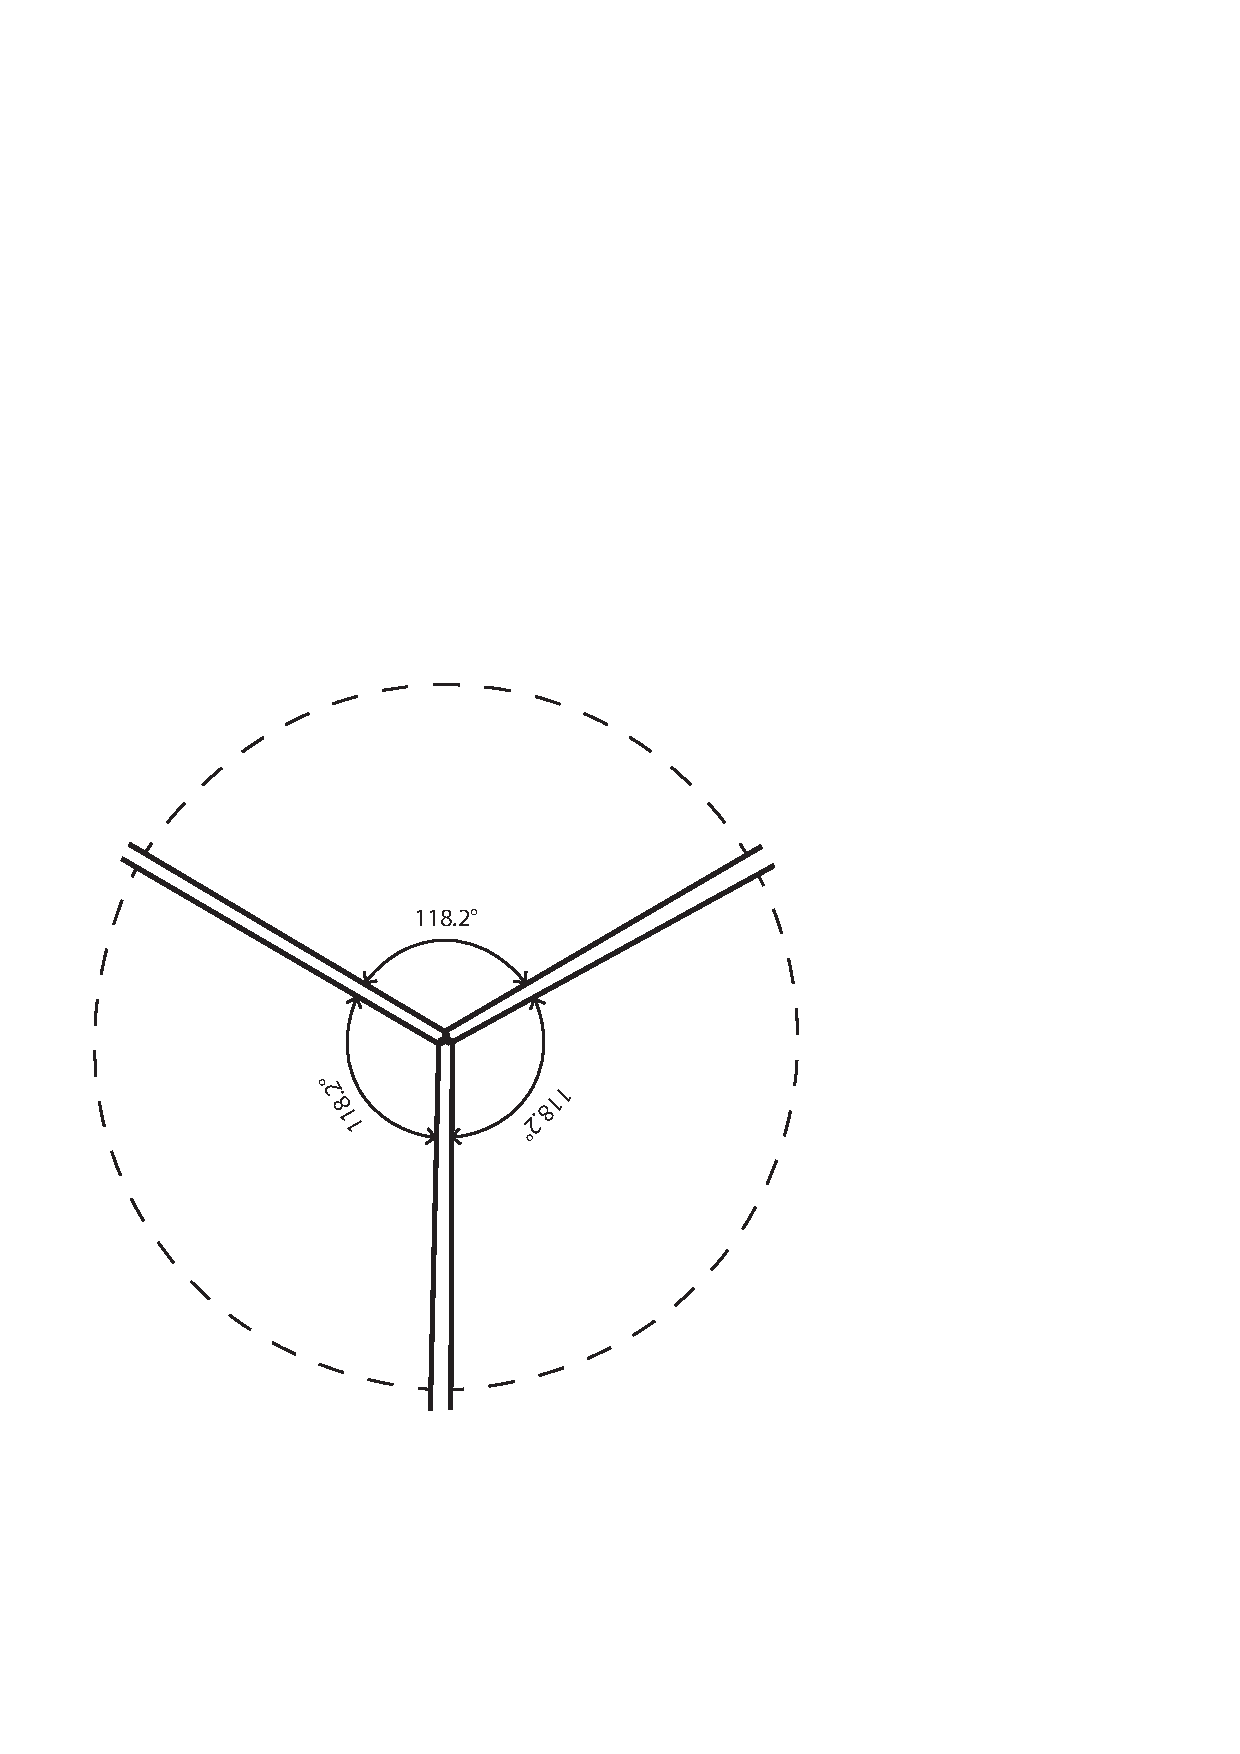
\includegraphics[width=0.4\textwidth]{./img/3-gopro-setup}}}\hfill
	\subfloat[implementation]{\label{fig:gopro-mdright}{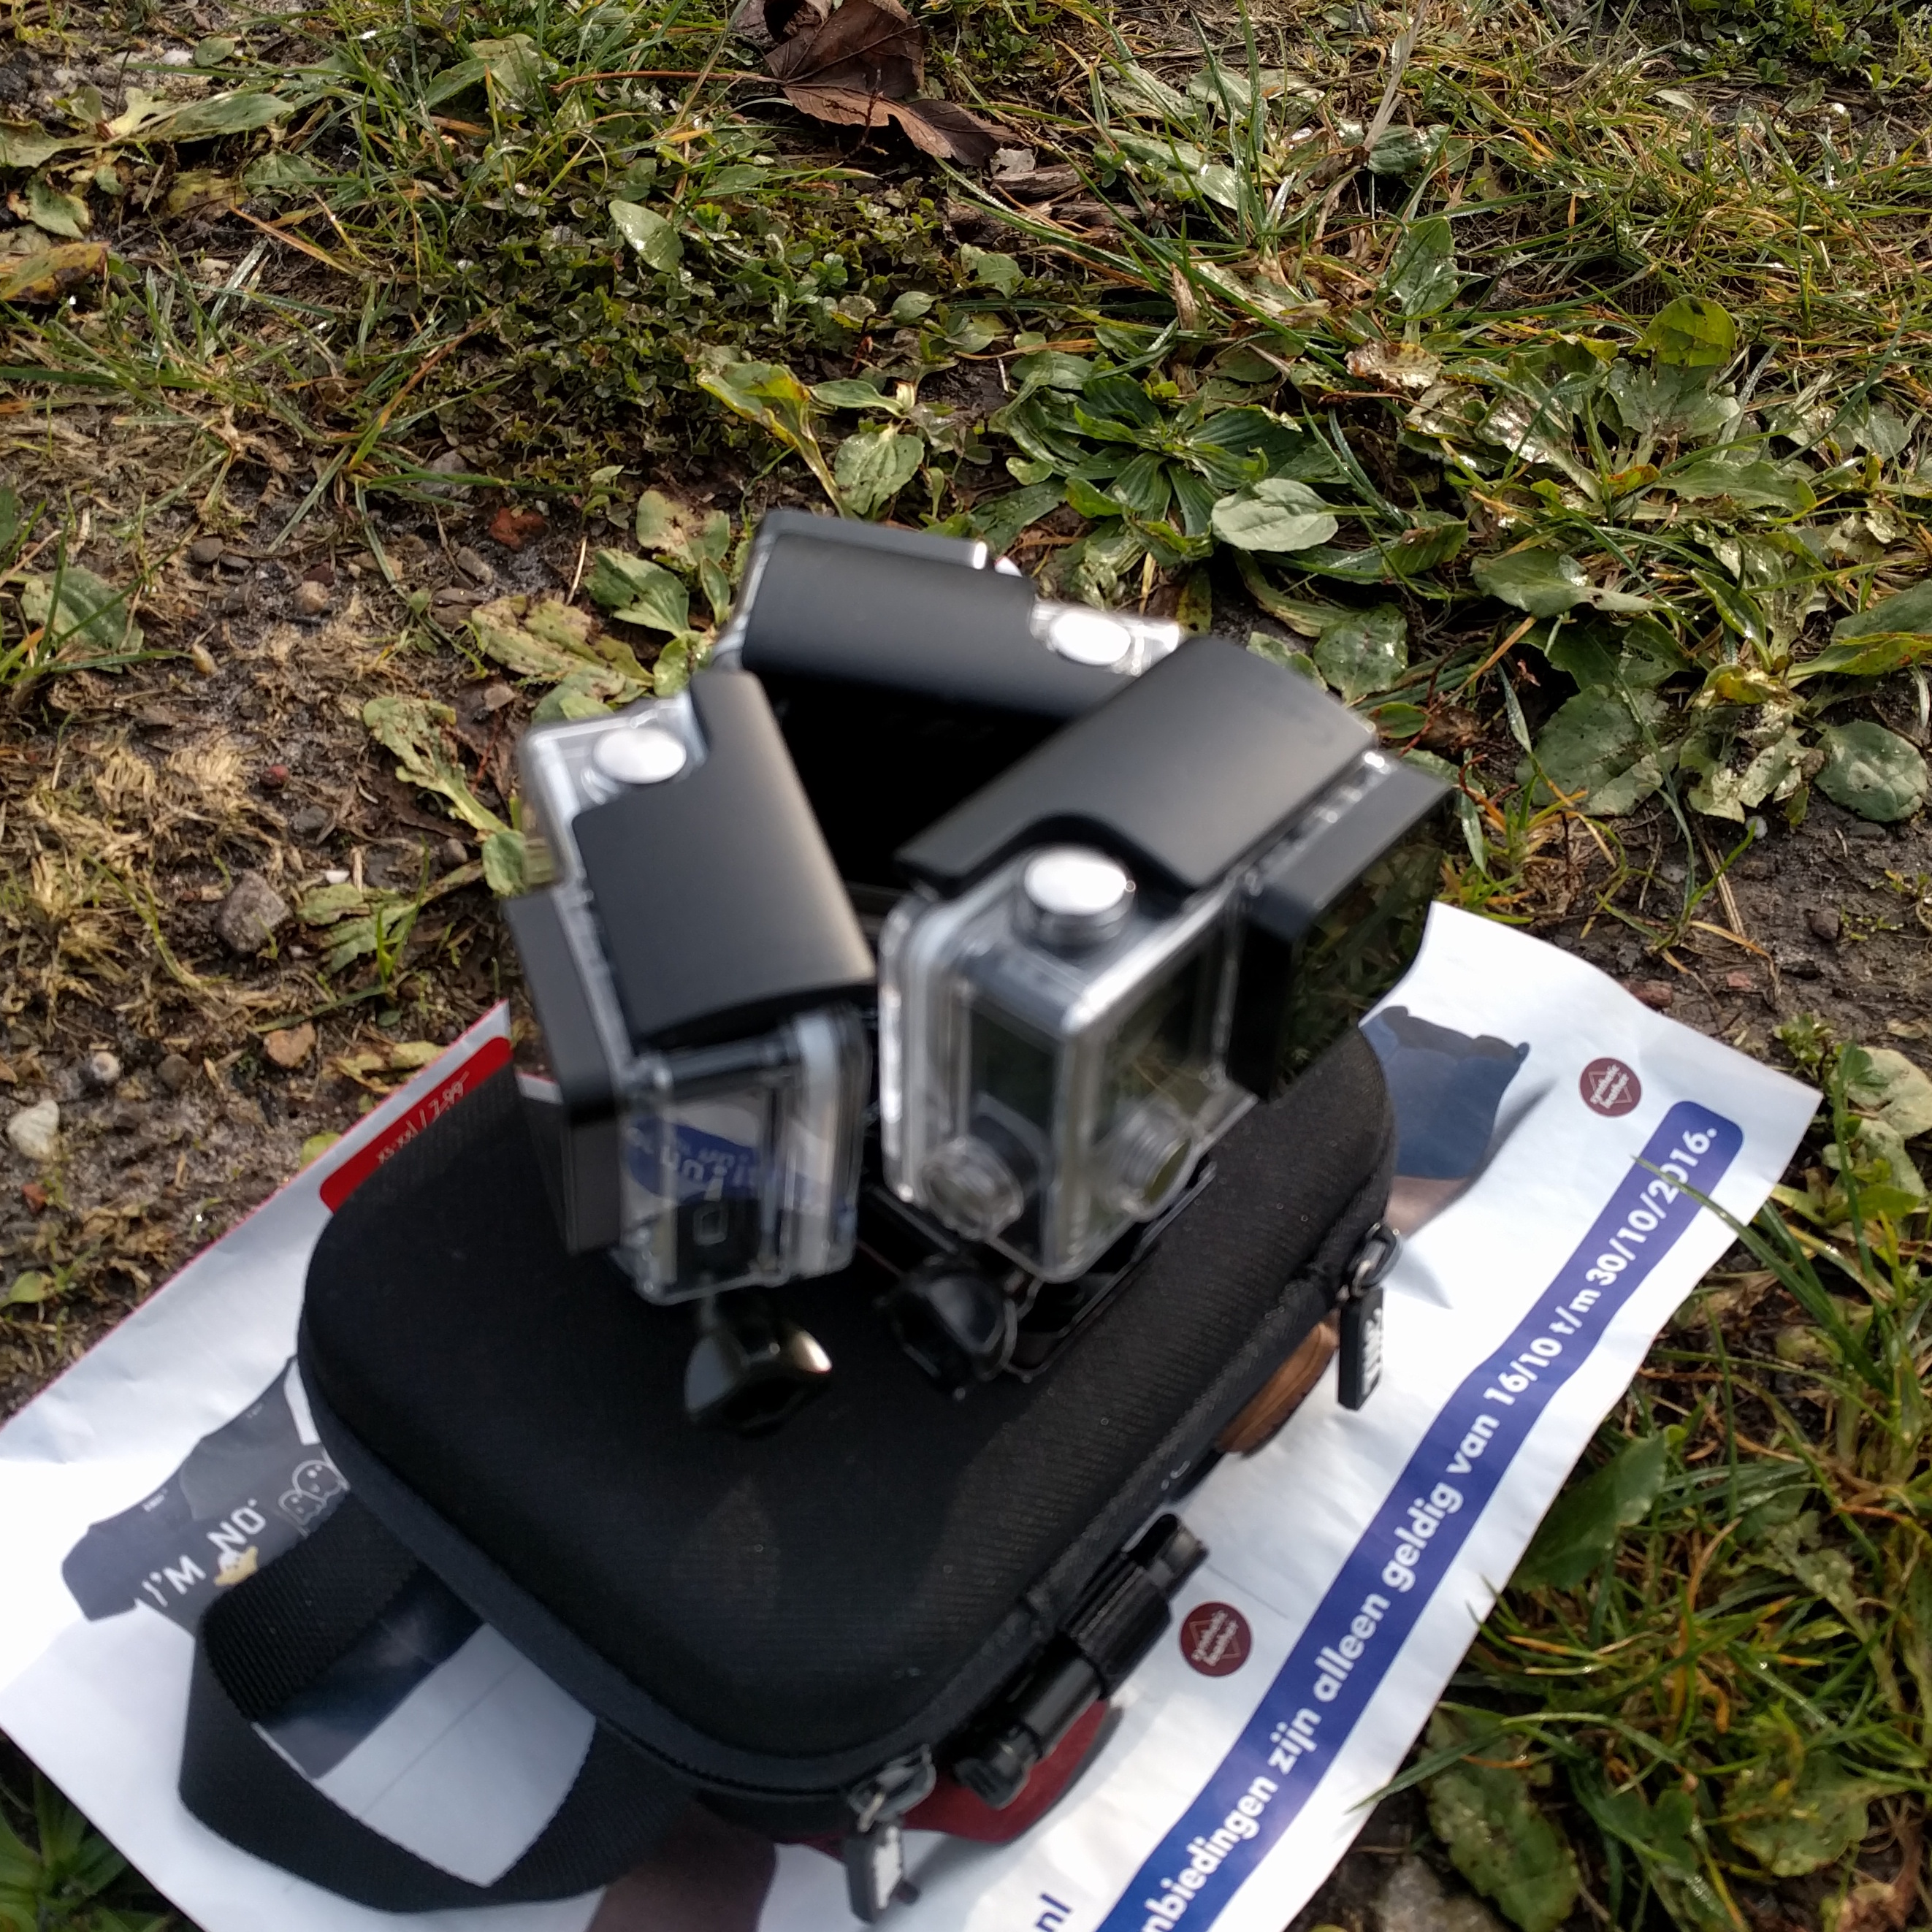
\includegraphics[width=0.4\textwidth]{./img/3-gopro-setup-pict}}}
	\caption{GoPro arrangement to achieve 360 degrees of horizontal \ac{FOV}.}
	\label{fig:gopro-placement}
	\end{figure}

	% setup, picture or vide, why?
	We use GoPro\footnote{\url{https://gopro.com}} Hero4 silver wide-angle action camera to get the photographic image. According to GoPro technical specifications~\cite{goprofieldofview}, its maximum horizontal \ac{FOV} is 118.2 degrees in 16$x$9 wide mode with 17.2mm focal length. Thus, to achieve 360 degrees of \ac{FOV} we use three GoPro cameras positioned in circular arrangement, as depicted in Figure~\ref{fig:gopro-placement}. Although some blind spots are still present, this setup is still able to capture objects within intended range.

	% we use timelapse, why: battery and memory limit
	We employ time-lapse photography technique to capture the surroundings in preference to normal video capture. In this technique we capture a still image in each five seconds, resulting 12 still images in each minute. We do not employ video recording to conserve GoPro battery. As stated in GoPro technical specification of battery life~\cite{goprobattery}, estimated battery life of taking video is roughly two hours, while our experiment is planned to be more than two hours (plus back-up time). We consider changing battery during data collection is impractical. Moreover, taking time-lapse images would increasingly save more data storage.
	
	In the end, we manually do head counting based on captured images grouped in each time interval. We make sure that one person is counted once to avoid counting the same person multiple times.

\subsection{Smartphone Sensor Utilization} % (fold)
\label{sub:smartphone_sensor_utilization}
We only use WiFi and microphone as sensors because those sensors are able to perceive the surroundings no matter how the smartphone is operated and positioned. This means that the passive monitoring process can still running in background regardless how user use the smartphone. In the other hand, camera based approach requires the smartphone to be positioned accordingly to be able to capture appropriate images for crowd counting.

	\subsubsection{WiFi scanning} % (fold)
	\label{ssub:wifi_scanning}
	Ideally we use probe request based crowd estimation, as discussed in Section~\ref{ssub:probe_request_based_estimation}, directly in the smartphone. However, this is not possible due to restriction in the mobile operating system. Probe request based estimation only works in WiFi monitor mode~\cite{thesis052,thesis079} and monitor mode is only accessible if the smartphone is rooted, jailbroken, or installed in custom \ac{ROM}, which is considered as illegal in most countries~\cite{rootjailbreak}.
	
	Hence, we count the available \ac{AP} nearby and observe its signal strength in place of unique \ac{MAC} address counting in probe request packets. We take note of \ac{AP}'s \ac{BSSID}, which is unique and based on \ac{MAC} address. We are not particularly interested in \ac{AP}'s \ac{SSID} because there might be multiple \ac{AP}s with the same \ac{SSID}. We measure the signal strength of the \ac{AP} in \ac{RSSI}.

	\subsubsection{Ambient Noise Recording} % (fold)
	\label{ssub:ambient_noise_recording}
	In addition to WiFi scanning we also record the ambient noise to perceive nearby condition. We assume that more crowded locations will have high ambient noise, while less crowded locations will have low ambient noise. We measure the ambient noise in decibels (dB). Moreover, we implement speaker count algorithm based on unsupervised learning method proposed by Xu et al~\cite{thesis067}. This approach will estimate how many persons are speaking in the audio recording.

\subsection{Location and Timing} % (fold)
\label{sub:location_and_timing}
To obtain wide range of data, we select four different locations that represent low and high crowd density as well as indoor and outdoor location. We plan to do our experiment where WiFi \ac{AP} use is not restricted, i.e., people are free to set up their own WiFi \ac{AP} in anyway they prefer. Some locations where the use of WiFi is restricted exist, for instance, University of Groningen complex. In the university complex, \verb|eduroam| is the only the official available \ac{AP} and the occupants are discouraged to install their own \ac{AP}. Thus, making this not suitable for our research. Table~\ref{tab:location-summary} summarizes our location selection.

To save GoPro battery, we select 30 minutes as the scanning duration in each location. As we are picking four different locations, this would sum up to two hours of image capture. We also select daytime as the preferred scanning time because that is the time when most crowd are observable.

\begin{table}[]
\centering
\caption{Summary of location and selection for the experiment}
\label{tab:location-summary}
\begin{tabular}{llll} \toprule
Location                  & Type    & Crowd Level & Scanning Time \\ \midrule
Remote area               & outdoor & low         & 11:00-11:30   \\
Home                      & indoor  & low--medium  & 08:15-08:45   \\
Paddepoel shopping center & indoor  & medium--high & 14:45-15:15   \\
Grote markt               & outdoor & high        & 12:00-12:30  \\ \bottomrule
\end{tabular}
\end{table}

% where is it, the maximum visitor [cite] where the scanner sit, is it indoor or outdoor.

% remote
Speaking of the location selection, remote area is a far-off outdoor location located in Paddepoelsterweg, Groningen. The surroundings are mostly trees and grasses. No visible buildings or dwellings exist but there is only a narrow asphalt pathway where sometimes people or vehicles pass by. Approximately no more than 5 individuals are present at the same time. We carry out the experiment in this area during daytime, from 11:00 to 11:30.

% home
Aside from the remote area where the crowd is less likely to be observed, we conduct a data collection at home during breakfast time, from 08:15 to 08:45. This indoor location is located at Planetenlaan 264, Groningen. Currently, there are only 6 inhabitants living in the house. However, people sometimes pass by in front of the house and they might influence the measurement result.

% paddepoel
Padeppoel shopping center is an indoor shopping center located in Paddepoel district, Groningen. The shopping center, which is 14.920 m\textsuperscript{2} in size, holds around 90 shops~\cite{paddepoelstat}. According to statistics~\cite{paddepoelstat}, it has approximately 90.000 visitors per week. We perform the experiment during the peak hours, which is from 14:45 to 15:15.

% grote markt
Grote markt is a open city square which is located in the center of Groningen city. This location is able to hold roughly 8000 visitors at the same time, according to the official government statement~\cite{GemeenteGroningen2016}. We are planning to do data collection in Grote Markt around mid day, from 12:00 to 12:30.

To see the variance between days, we plan to do the experiment in four days, ranging from weekdays to weekend. We start the experiment in Wednesday and finish it in Saturday. We stick to the same schedule for each location.

\subsection{Scanning Mechanism} % (fold)
\label{sub:scanning}
In summary, we are using three inputs to collect and to perceive the surroundings, namely WiFi, microphone, and wide-angle camera. The data collection process is split into several small cycles of $x$ minutes to avoid biased result caused by randomized \ac{MAC} address. The $x$ will be determined by the \ac{MAC} address randomization experiment described in Section~\ref{sec:mac_address_randomization}. We keep repeating the cycle until we reach 30 minutes. Figure~\ref{fig:sensor-measurement} depicts the description of each cycle.

\begin{figure}[ht]
	\centering
	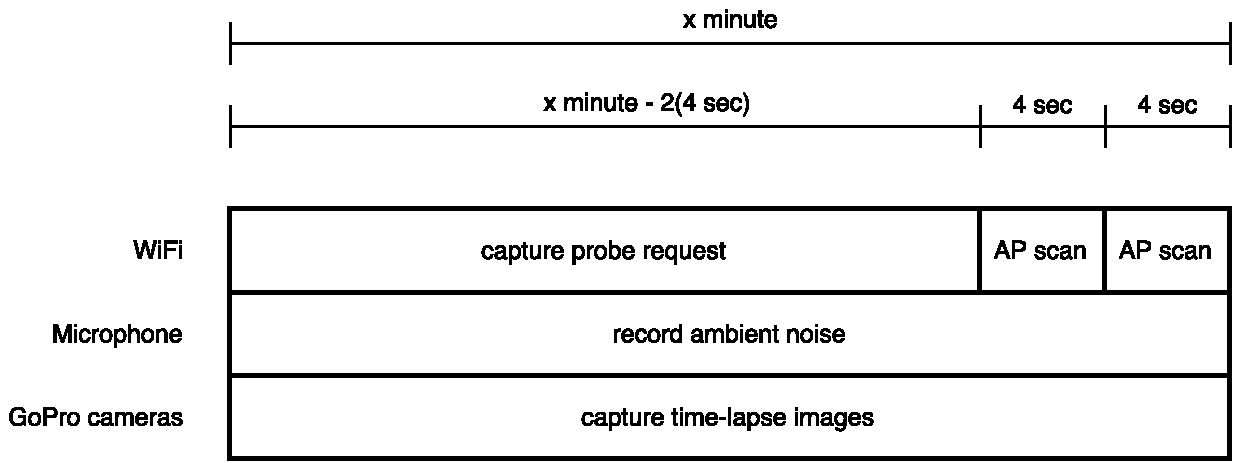
\includegraphics[width=\textwidth]{./img/3-scanning-mechanism}
	\caption{Sensor measurement in each cycle.}
	\label{fig:sensor-measurement}
\end{figure}

% design
As depicted in Figure~\ref{fig:sensor-measurement}, we work with WiFi to capture the probe request and count the number of available \ac{AP}. We cannot perform these tasks simultaneously, because capturing probe request must be carried out in the WiFi monitor mode. Monitor mode is one of the seven modes, namely master (acting as an \ac{AP}), managed (acting as a WiFi client), ad-hoc, mesh, repeater, and promiscuous, that 802.11 WiFi cards can operate in~\cite{thesis082}. Being in monitor mode, the WiFi card is disconnected from any wireless networks. Thus, we decide to firstly capture probe request before counting the available \ac{AP}. We count the available \ac{AP} twice to achieve better stability. Both microphone and GoPro cameras continuously recording ambient noise and capturing time-lapse images in each cycle.

% technical, both hardware and software
We use Apple MacBook Air, with built-in WiFi card and microphone, as a WiFi scanning and audio recording device. To capture probe request, we use \verb|tcpdump|\footnote{\url{http://www.tcpdump.org}}, a free packet analyzer that runs under the command line, and we use console based Apple's AirPort utility, a software designed by Apple to manage WiFi network, to count available access point. The output of probe request capture is \verb|.pcap| file, a standard file for capturing network traffic. \ac{AP} counting results in plain text files. We work with console based audio editing software, Sound Exchange\footnote{\url{http://sox.sourceforge.net}}, to record the ambient noise to \verb|.wav| file format.

To automate the WiFi scanning and audio recording process, we write a bash script\footnote{Bash script is a list of Bash commands that run on console based application to execute particular tasks.}. We label the resulting log files in the corresponding timestamp and location. Our code is publicly available online\footnote{\url{https://github.com/gtrdp/masters-thesis-guntur}}.

\subsubsection{Effect of Scanning Time} % (fold)
\label{ssub:effect_of_scanning_time}
In addition to the previous experiment which is particularly aimed to see the variance between days, we also conduct an experiment aiming at seeing the variance between scanning time. In this experiment we select Grote Markt Groningen as the scanning location with four different scanning time, taken at
\begin{enumerate*}[label={\alph*)},font={\color{red!50!black}\bfseries}]
  \item 09:00,
  \item 12:00,
  \item 15:00,
  \item and 18:00
\end{enumerate*},
in the same day. The rest of the experimental setup of this process remains the same as previous experiment. However, we do not employ GoPro time-lapse image capture.








\section{Data Extraction} % (fold)
\label{sec:data_extraction}
The experiments mentioned previously will produce different formats of hundreds of raw files that need further processing to give us more insights. The files are, namely, \verb|.txt| for \ac{AP} list, \verb|.pcap| for captured probe request packets, \verb|.wav| for recorded ambient noise, and \verb|.jpeg| for time-lapse images. Each file format needs different treatment to extract the data. Table~\ref{tab:sensor-parameters} summarizes all sensor readings and the extracted parameters.

\begin{table}[]
\centering
\caption{Smartphone sensor readings and the extracted parameters}
\label{tab:sensor-parameters}
\begin{tabular}{llll}\toprule
Sensor     & File format & Extracted parameter & Extraction method\\ \midrule
WiFi       & \verb|.pcap| & unique \ac{MAC} addresses     & text processing \\
WiFi       & \verb|.txt| & \ac{AP} signal strength     & text processing \\
WiFi       & \verb|.txt| & \ac{AP} count            & text processing \\
Microphone & \verb|.wav| & speaker count       & machine learning \\
Microphone & \verb|.wav| & peak level          & audio processing \\
Microphone & \verb|.wav| & root mean square    & audio processing \\
GoPro cameras & \verb|.jpg| & head count       & manual counting\\
\bottomrule
\end{tabular}
\end{table}

\subsection{WiFi Raw Data Extraction} % (fold)
\label{sub:wifi_raw_data_extraction}
The WiFi based data collection result consists of two types of file, namely \verb|.txt| file for \ac{AP} list from AirPort sensing, and \verb|.pcap| file for captured probe request packets from \verb|tcpdump| sensing. As shown in Table~\ref{tab:sensor-parameters}, we extract the number of available \ac{AP} and the mean of \ac{AP}'s signal strength from this file, while the number of unique device is derived from the \verb|.pcap| file. Each cycle produces two individual \verb|.txt| and \verb|.pcap| labeled in its corresponding timestamp.

Figure~\ref{fig:ap-list-example} and~\ref{fig:probe-request-example} display the example of sensed \ac{AP} list and captured probe request respectively. From the \ac{AP} list depicted in Figure~\ref{fig:ap-list-example} we are interested in \ac{BSSID} column and \ac{RSSI} column to count the \ac{AP} and measure the signal strength. From the captured probe request packets, as depicted in Figure~\ref{fig:probe-request-example}, we take note on the \ac{SA}. We develop a text processing program written in Python script to extract preferred elements. We plot the result to scatter plot using \verb|matplotlib| package in Python~\cite{Hunter:2007}.


anonymized, explain.

% example of airport scanning result
\begin{figure}[ht]
	\centering
\begin{verbatim}
                SSID BSSID             RSSI CHANNEL 
               Ziggo 6c:aa:b3:27:72:ac -84  140     
               Ziggo 6c:aa:b3:26:af:bc -87  140     
       Ziggo22211-5G 0c:54:a5:b8:25:e8 -84  136,-1  
             eduroam c4:10:8a:60:d4:7c -84  132,+1  
 Draadloos Groningen c4:10:8a:20:d4:7c -84  132,+1  
       Ziggo21616-5G 60:02:92:11:4d:e6 -87  128,-1  
               Ziggo 6c:aa:b3:26:af:0c -86  116,+1  
             OneTeam e2:55:6d:20:30:96 -85  108,+1  
   WEEKDAY Free WiFi e2:55:6d:20:30:92 -85  108,+1  
\end{verbatim}
	\caption{Example of \ac{AP} list.}
	\label{fig:ap-list-example}
\end{figure}

% example of pcap file readings
\begin{figure}[ht]
\centering
\begin{verbatim}
BSSID:ff:ff:ff:ff:ff:ff DA:ff:ff:ff:ff:ff:ff SA:ec:1f:72:10:44:01
BSSID:ff:ff:ff:ff:ff:ff DA:ff:ff:ff:ff:ff:ff SA:0a:0f:c6:e5:e0:cb
BSSID:ff:ff:ff:ff:ff:ff DA:ff:ff:ff:ff:ff:ff SA:2e:60:57:70:d3:eb
\end{verbatim}
\caption{A fragment of captured probe request packet.}
\label{fig:probe-request-example}
\end{figure}

\subsection{Recorded Ambient Noise Extraction} % (fold)
\label{sub:recorded_ambient_noise_extraction}
We extract single ambient noise recording \verb|.wav| file to three independent measurements, namely the \ac{PKLV}, \ac{RMS}, and speaker count. We use the same audio processing program as ambient noise recording process, namely Sound Exchange, to extract the \ac{PKLV} and \ac{RMS} from the \verb|.wav| file, while we use unsupervised learning method proposed by Xu et al.~\cite{thesis067}, namely Crowd++, to infer the number of speaker count.

The \ac{PKLV} is the highest value of a total waveform, while \ac{RMS} is the effective value or the mean. The \ac{PKLV} and \ac{RMS} are both measured in decibels (dB). As a performance test of Crowd++, we perform speaker count check in several audio recordings with known ground truth. The recordings are a commencement speech (1 speaker), pop duets (2 speakers), and acapella (5 speakers). We will use the result as a consideration whether this speaker method is reliable.

% Crowd++ Using the code from the original version.
% Remove unrelated code block, such as the relation with smartphone things: battery, calibration (because we do not use semisupervised learning based on the owner voice) etc.
% The code also uses Java Speech Toolkit (JSTK) from Speech Group at Informatik 5, Univ. Erlangen-Nuremberg, GERMANY.
% % https://github.com/sikoried/jstk
% Most time spent on debugging the code.
% Crowdpp also uses YIN pitch tracking algorithm:
% % http://recherche.ircam.fr/equipes/pcm/cheveign/ps/2002_JASA_YIN_proof.pdf
% Finally got the code to work, bug found in file format and feature extraction (delete the feature after completed, otherwise the next process will append it which will cause Exception)
% Found SoX, an audio recorder (and even more) for sound recording:
% % http://sox.sourceforge.net/sox.html
% Explain the audio result: what is pklv and rms.

\subsection{Manual Head Counting} % (fold)
\label{sub:manual_head_counting}
We firstly collect all time-lapse images taken in different location from the three GoPro cameras. Then, we group each time-lapse image separately to the corresponding cycle and camera. We then manually do head counting based on those images and apply pattern recognition (manually) to avoid counting the same object that appears more than once multiple times. The result is a total head count of a cycle per location.
	







% Good conclusion brings an intro to the next chapter.
This chapter presents the method that we plan to execute the experiments, started by \ac{MAC} address randomization investigation, then followed by an examination of the correlation between the people count and the smartphone sensor readings, and ended with how we extract the data from the raw log files. The next chapter will tell us the result of each experiment.

%*****************************************
%*****************************************
%*****************************************
%*****************************************
%*****************************************
